\documentclass[tikz]{standalone}
\usepackage[compat=1.1.0]{tikz-feynman}
% documentation
%https://jpellis.me/projects/tikz-feynman/tikz-feynman/tikz-feynman.pdf

\begin{document}
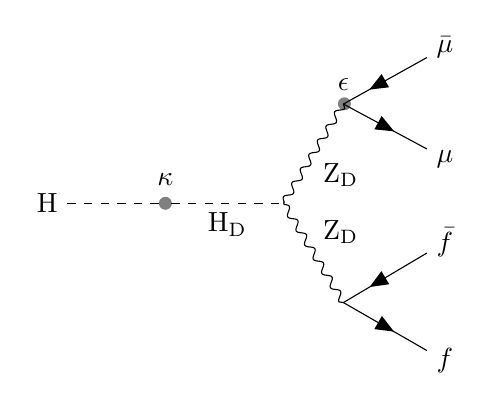
\begin{tikzpicture}
	\begin{feynman}
	\vertex(a){\({\rm H}\)};
	\vertex[right=of a, dot, style = gray] (b){};
	\vertex[above=3 mm of b] {\(\kappa\)}; %simple trick to draw vertex labels
	\vertex[right=of b   ] (c);
	\vertex[above right=of c,  yshift =  1.5mm, xshift = -3.4mm, dot, style = gray]{}; %simple trick to draw vertex labels
    \vertex[above right=of c,  yshift =  2mm, xshift = -3mm] (c1);
	\vertex[below right=of c,  yshift = -2mm, xshift = -3mm] (c2);
	\vertex[above= 0.5 mm of c1] {\(\epsilon\)}; %simple trick to draw vertex labels
	\vertex[above right=of c1, yshift = -6mm] (f1){\(\bar{\mu}\)};
	\vertex[below right=of c1, yshift =  6mm] (f2){\(\mu\)};
	\vertex[above right=of c2, yshift = -6mm] (f3){\(\bar{f}\)};
	\vertex[below right=of c2, yshift =  6mm] (f4){\(f\)};
    %\vertex[above right=of c2, yshift = -9mm] (f3){};
	%\vertex[below right=of c2, yshift =  9mm] (f4){};
	\diagram* {
		(a)-- [scalar] (b) -- [scalar, edge label'=\({\rm H_D}\)] (c) -- [boson,edge label'=\({\rm Z_D}\)] (c1),
		(c)-- [boson,edge label=\({\rm Z_D}\)] (c2),
		(c1)--[anti fermion] (f1),
		(c1)--[fermion] (f2),
		(c2)--[anti fermion] (f3),
		(c2)--[fermion] (f4),
		};
	\end{feynman}
\end{tikzpicture}

\end{document}
